\section{Wymagania}
W tej sekcji znajduje się lista wymagań, jakie spełniać powinien budowany system. Podane są~one z~podziałem na~dwie kategorie. Pierwsza to wymagania funkcjonalne -- określające funkcjonalności systemu oraz sposoby ich użycia. Natomiast druga to~wymagania niefunkcjonalne, które opisują ilościowe i~jakościowe warunki działania systemu.

\subsection{Wymagania funkcjonalne}
\subsubsection{Użytkownicy}
Wymagania funkcjonalne dotyczące zarządzaniem użytkownikami w~systemie.
\begin{itemize}
  \item logowanie do aplikacji,
  \item wyświetlanie listy użytkowników,
  \item dodawanie nowego użytkownika,
  \item edycja danych użytkownika,
  \item usunięcie użytkownika.
\end{itemize}

\subsubsection{Konta}
Wymagania funkcjonalne dotyczące zarządzaniem kontami pieniężnymi w~systemie.
\begin{itemize}
  \item wyświetlanie listy kont,
  \item dodawanie nowego konta,
  \item edycja danych konta,
  \item usunięcie konta.
\end{itemize}

\subsubsection{Transakcje}
Wymagania funkcjonalne dotyczące zarządzaniem transakcjami w~systemie.
\begin{itemize}
  \item wyświetlanie listy transakcji,
  \item dodawanie nowej transakcji,
  \item edycja danych transakcji,
  \item usunięcie transakcji.
\end{itemize}

\subsubsection{Budżet}
Wymagania funkcjonalne dotyczące zarządzaniem budżetami w~systemie.
\begin{itemize}
  \item wyświetlenie budżetów ustawionych w~systemie,
  \item ustawienie budżetu dla określonego użytkownika,
  \item modyfikacja budżetu sumarycznego dla wszystkich użytkowników,
  \item modyfikacja budżetu określonego użytkownika,
  \item usunięcie budżetu określonego użytkownika.
\end{itemize}

\subsubsection{Raporty}
Wymagania funkcjonalne dotyczące generowania raportów w~systemie.
\begin{itemize}
  \item konfiguracja raportu,
  \item wyświetlanie raportu,
  \item zapisywanie raportu do~pliku.
\end{itemize}

\subsubsection{Opis przypadków użycia -- użytkownicy}

\begin{figure}[H]
  \centering
  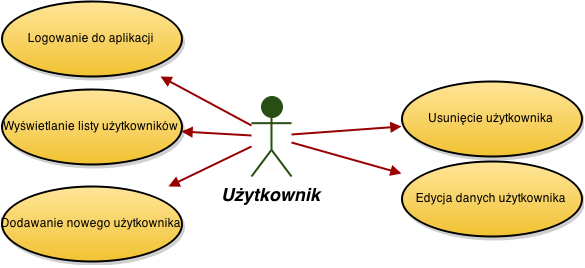
\includegraphics[width=0.7\textwidth]{images/przypadki_uzytkownik.png}
  \caption{Diagram przypadków użycia związanych z~kontami użytkowników.}
\end{figure}

\paragraph{Dodawanie nowego użytkownika\newline}
\label{par:register}

\textit{Opis słowny} -- niniejszy przypadek użycia umożliwia użytkownikowi stworzenie konta, poprzez które będzie miał
on dostęp do systemu.

\begin{longtable}{|p{5cm}|p{8cm}|}
  \hline \textbf{Aktor} & Użytkownik \\ \hline
  \textbf{Warunki początkowe} & Użytkownik nie jest zarejestrowany \\ \hline
  \textbf{Opis przebiegu interakcji} & Wybór strony z~rejestracją, wprowadzenie danych, kliknięcie przycisku,
  zatwierdzenie \\ \hline
  \textbf{Sytuacje wyjątkowe} & Niepoprawnie wprowadzone dane \\ \hline
  \textbf{Warunki końcowe} & Nowy użytkownik w~systemie \\ \hline
\end{longtable}

\noindent \textit{Scenariusz główny:}
\begin{enumerate}
  \item Użytkownik otwiera stronę ,,Logowanie/Rejestracja''.
  \item Użytkownik wybiera opcję ,,Rejestracja'' i~wprowadza niezbędne dane.
  \item Użytkownik naciska przycisk ,,Zarejestruj''.
  \item Aplikacja sprawdza wprowadzone dane.
  \item Jeżeli nie wystąpiły żadne błędy, system wysyła aktywacyjną wiadomość e-mail na adres wprowadzony przez użytkownika i~informuje go, aby go odebrał.
  \item Użytkownik otwiera wiadomość i~klika w~link aktywacyjny.
  \item Aplikacja rejestruje nowego użytkownika i~przekierowuje go do strony logowania.
\end{enumerate}

\noindent \textit{Scenariusz alternatywny -- niepoprawne dane:}
\begin{enumerate}
  \item[1-4.] Jak w~scenariuszu głównym.
  \item[5.] System wyświetla informacje o~wykrytym błędzie.
  \item[6.] Użytkownik poprawia wprowadzone dane i~naciska przycisk ,,Zarejestruj''.
  \item[7.] Powrót do kroku 4.~ze scenariusza głównego.
\end{enumerate}

\begin{figure}[H]
  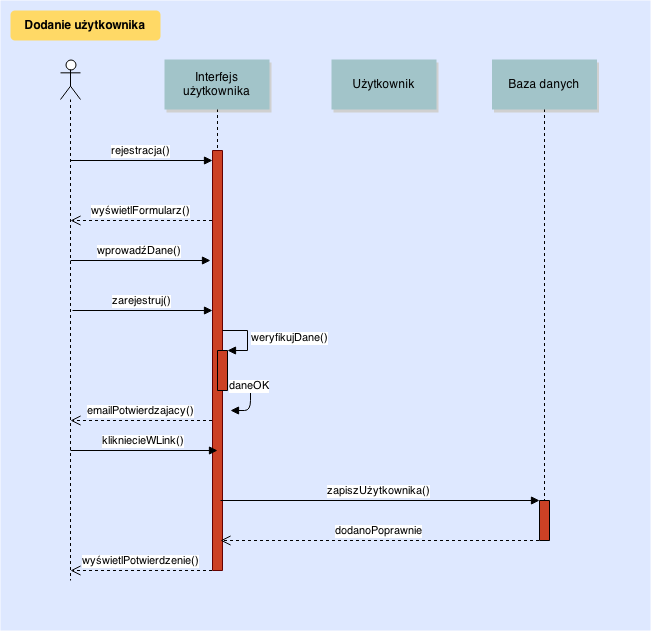
\includegraphics[width=\textwidth]{images/dodaj_uzytkownika.png}
  \caption{Diagram sekwencji dla przypadku użycia~\ref{par:register}~--~Dodawanie nowego użytkownika (scenariusz główny)}
\end{figure}

\newpage
\paragraph{Logowanie do~aplikacji\newline}
\label{par:login}

\textit{Opis słowny} -- niniejszy przypadek użycia umożliwia użytkownikowi zalogowanie się do systemu, dzięki czemu
będzie on miał dostęp do wszystkich funkcjonalności.

\begin{longtable}{|p{5cm}|p{7cm}|}
  \hline \textbf{Aktor} & Użytkownik \\ \hline
  \textbf{Warunki początkowe} & Użytkownik jest zarejestrowany \\ \hline
  \textbf{Opis przebiegu interakcji} & Wybór strony z~logowaniem, wprowadzenie danych, kliknięcie przycisku \\ \hline
  \textbf{Sytuacje wyjątkowe} & Niepoprawnie wprowadzone dane \\ \hline
  \textbf{Warunki końcowe} & Użytkownik jest zalogowany \\ \hline
\end{longtable}

\noindent \textit{Scenariusz główny:}
\begin{enumerate}
  \item Użytkownik otwiera stronę ,,Logowanie/Rejestracja''.
  \item Użytkownik wybiera opcję ,,Logowanie'' i~wprowadza dane:~adres e-mail oraz hasło.
  \item Użytkownik naciska przycisk ,,Zaloguj''.
  \item Aplikacja sprawdza wprowadzone dane.
  \item Jeżeli para (e-mail,~hasło) znajduje się w~systemie, aplikacja przekierowuje użytkownika na docelową stronę.
\end{enumerate}

\noindent \textit{Scenariusz alternatywny -- niepoprawne dane:}
\begin{enumerate}
  \item[1-4.] Jak w~scenariuszu głównym.
  \item[5.] System wyświetla informacje o~wykrytym błędzie.
  \item[6.] Użytkownik poprawia wprowadzone dane i~naciska przycisk ,,Login''.
  \item[7.] Powrót do kroku 4.~ze scenariusza głównego.
\end{enumerate}

\begin{figure}[H]
  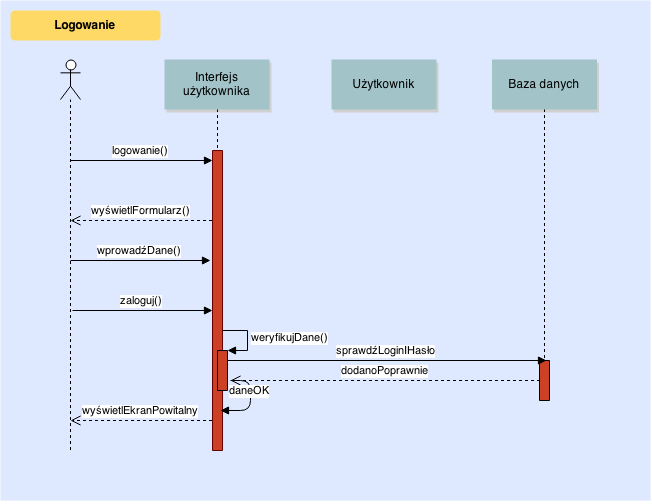
\includegraphics[width=\textwidth]{images/logowanie.png}
  \caption{Diagram sekwencji dla przypadku użycia~\ref{par:login}~--~Logowanie do aplikacji (scenariusz główny)}
\end{figure}

\paragraph{Wyświetlanie listy użytkowników\newline}
\label{par:userList}
Korzysta z~\ref{par:login}~--~Logowanie do~aplikacji.\\

\textit{Opis słowny} -- niniejszy przypadek użycia umożliwia użytkownikowi wyświetlenie listy użytkowników
korzystających z~systemu.

\begin{longtable}{|p{5cm}|p{7cm}|}
  \hline \textbf{Aktor} & Użytkownik \\ \hline
  \textbf{Warunki początkowe} & Użytkownik jest zalogowany \\ \hline
  \textbf{Opis przebiegu interakcji} & Wybór strony z~użytkownikami \\ \hline
  \textbf{Sytuacje wyjątkowe} & Użytkownik nie jest zalogowany \\ \hline
  \textbf{Warunki końcowe} & Wyświetlona lista użytkowników \\ \hline
\end{longtable}

\noindent \textit{Scenariusz główny:}
\begin{enumerate}
  \item Użytkownik otwiera stronę ,,Użytkownicy''.
  \item Jeśli użytkownik nie jest zalogowany, aplikacja wymaga zalogowania, inicjując~\ref{par:login}~--~Logowanie do~aplikacji.
  \item Aplikacja wyświetla użytkowników zarejestrowanych w~systemie.
\end{enumerate}

\begin{figure}[H]
  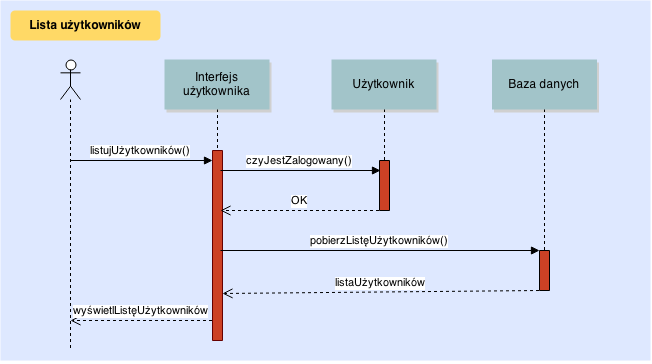
\includegraphics[width=\textwidth]{images/listuj_uzytkownikow.png}
  \caption{Diagram sekwencji dla przypadku użycia~\ref{par:userList}~--~Wyświetlanie listy użytkowników (scenariusz główny)}
\end{figure}

\paragraph{Edycja danych użytkownika\newline}
\label{par:editUser}
Korzysta z~\ref{par:login}~--~Logowanie do~aplikacji.\\

\textit{Opis słowny} -- niniejszy przypadek użycia umożliwia użytkownikowi edycję danych dotyczących jego profilu.

\begin{longtable}{|p{5cm}|p{7cm}|}
  \hline \textbf{Aktor} & Użytkownik \\ \hline
  \textbf{Warunki początkowe} & Użytkownik jest zalogowany \\ \hline
  \textbf{Opis przebiegu interakcji} & Wybór strony z~profilem, wprowadzenie danych, kliknięcie przycisku, zatwierdzenie \\ \hline
  \textbf{Sytuacje wyjątkowe} & Błędnie wprowadzone dane \\ \hline
  \textbf{Warunki końcowe} & Dane użytkownika zaktualizowane w~systemie \\ \hline
\end{longtable}

\noindent \textit{Scenariusz główny:}
\begin{enumerate}
  \item Użytkownik loguje się do aplikacji, tak jak w~scenariuszu~\ref{par:login}~--~Logowanie do aplikacji.
  \item Użytkownik otwiera stronę ,,Profil''.
  \item Użytkownik naciska przycisk ,,Edytuj profil''.
  \item Aplikacja wyświetla okno zawierające dane użytkownika.
  \item Użytkownik edytuje imię, nazwisko, adres e-mail lub hasło i~naciska przycisk ,,Zapisz''.
  \item System prosi użytkownika o~potwierdzenie zmiany poprzez wpisanie starego hasła.
  \item System weryfikuje wprowadzone dane.
  \item Jeżeli dane są prawidłowe, system edytuje dane użytkownika.
\end{enumerate}

\noindent \textit{Scenariusz alternatywny -- niepoprawne dane:}
\begin{enumerate}
  \item[1-7.] Jak w~scenariuszu głównym.
  \item[8.] System wyświetla informacje o~wykrytym błędzie.
  \item[9.] Użytkownik poprawia dane i~naciska przycisk ,,Zapisz''.
  \item[10.] Powrót do kroku 7.~ze scenariusza głównego.
\end{enumerate}

\begin{figure}[H]
  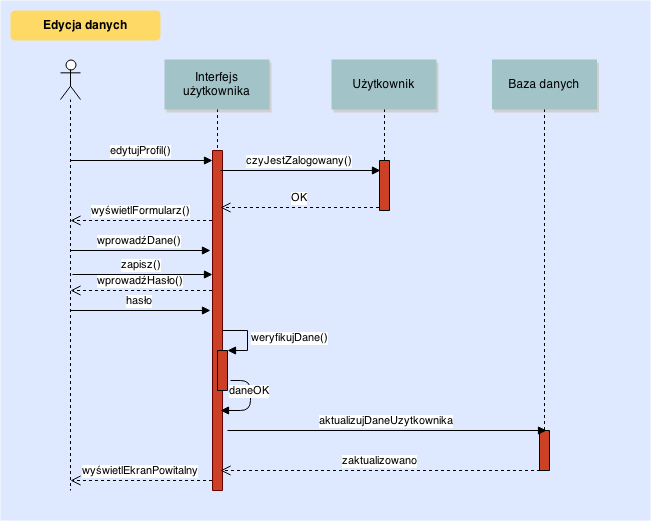
\includegraphics[width=\textwidth]{images/edytuj_uzytkownika.png}
  \caption{Diagram sekwencji dla przypadku użycia~\ref{par:editUser}~--~Edycja danych użytkownika (scenariusz główny)}
\end{figure}

\newpage
\paragraph{Usunięcie użytkownika\newline}
\label{par:deleteUser}
Korzysta z~\ref{par:login}~--~Logowanie do~aplikacji.\\

\textit{Opis słowny} -- niniejszy przypadek użycia umożliwia użytkownikowi skasowanie swojego profilu z~systemu.

\begin{longtable}{|p{5cm}|p{7cm}|}
  \hline \textbf{Aktor} & Użytkownik \\ \hline
  \textbf{Warunki początkowe} & Użytkownik jest zalogowany \\ \hline
  \textbf{Opis przebiegu interakcji} & Wybór strony z~profilem, wprowadzenie danych, kliknięcie przycisku \\ \hline
  \textbf{Sytuacje wyjątkowe} & Błędnie wprowadzone dane \\ \hline
  \textbf{Warunki końcowe} & Skasowanie użytkownika z~systemu i~wylogowanie \\ \hline
\end{longtable}

\noindent \textit{Scenariusz główny:}
\begin{enumerate}
  \item Użytkownik loguje się do aplikacji, tak jak w~scenariuszu~\ref{par:login}~--~Logowanie do aplikacji.
  \item Użytkownik otwiera stronę ,,Profil''.
  \item Użytkownik naciska przycisk ,,Usuń użytkownika''.
  \item System prosi użytkownika o~potwierdzenie decyzji poprzez wpisanie hasła i~naciśnięcie przycisku ,,Usuń''.
  \item System weryfikuje poprawność hasła.
  \item Jeżeli hasło jest zgodne, aplikacja usuwa informacje o~użytkowniku i~następuje wylogowanie.
\end{enumerate}

\noindent \textit{Scenariusz alternatywny -- użytkownik nie potwierdza decyzji:}
\begin{enumerate}
  \item[1-5.] Jak w~scenariuszu głównym.
  \item[6.] Użytkownik nacisnął przycisk ,,Anuluj''.
  \item[7.] System powraca do strony ,,Profil''.
\end{enumerate}

\noindent \textit{Scenariusz alternatywny -- niepoprawne dane:}
\begin{enumerate}
  \item[1-5.] Jak w~scenariuszu głównym.
  \item[6.] System wyświetla informację o~wykrytym błędzie.
  \item[7.] Użytkownik poprawia hasło i~naciska przycisk ,,Usuń''.
  \item[7.] Powrót do kroku 5.~ze scenariusza głównego.
\end{enumerate}

\begin{figure}[H]
  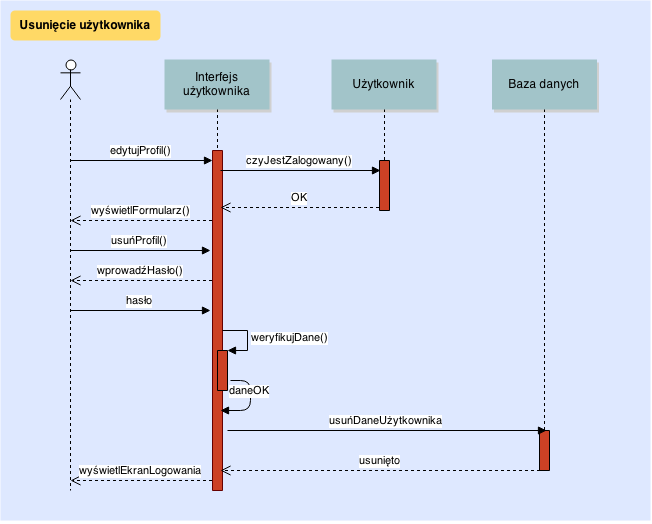
\includegraphics[width=\textwidth]{images/usun_uzytkownika.png}
  \caption{Diagram sekwencji dla przypadku użycia~\ref{par:deleteUser}~--~Usunięcie użytkownika (scenariusz główny)}
\end{figure}

\subsubsection{Opis przypadków użycia -- konta}

\begin{figure}[H]
  \centering
  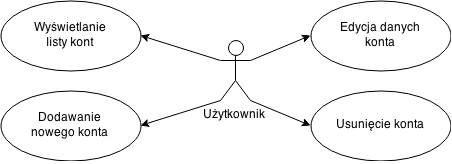
\includegraphics[width=0.9\textwidth]{images/use-cases-accounts.png}
  \caption{Diagram przypadków użycia związanych z~zarządzaniem kontami.}
\end{figure}

\newpage
\paragraph{Wyświetlanie listy kont\newline}
\label{par:accountsView}
Korzysta z~\ref{par:login}~--~Logowanie do~aplikacji.\\
\indent Funkcja generalizująca dla~\ref{par:accountCreate},~\ref{par:accountEdit} oraz~\ref{par:accountDelete}.\\

\textit{Opis słowny} -- niniejszy przypadek użycia umożliwia użytkownikowi wyświetlenie listy kont, które są~do~niego przypisane w~programie. Dzięki temu może on~łatwo nimi zarządzać oraz monitorować ich stan.\\

\begin{tabular}{|l|l|}
  \hline \textbf{Aktor} & Użytkownik \\ \hline
  \textbf{Warunki początkowe} & Użytkownik jest zalogowany \\ \hline
  \textbf{Opis przebiegu interakcji} & Wybór strony z~kontami \\ \hline
  \textbf{Sytuacje wyjątkowe} & Brak \\ \hline
  \textbf{Warunki końcowe} & Wyświetlona lista posiadanych kont \\ \hline
\end{tabular}\\\\

\noindent \textit{Scenariusz główny:}
\begin{enumerate}
  \item Użytkownik otwiera stronę ,,Konta''.
  \item Jeśli użytkownik nie jest zalogowany, aplikacja wymaga zalogowania, inicjując~\ref{par:login}~--~Logowanie do~aplikacji.
  \item Aplikacja wyświetla konta należące do zalogowanego użytkownika.
\end{enumerate}

\begin{figure}[H]
  \centering
  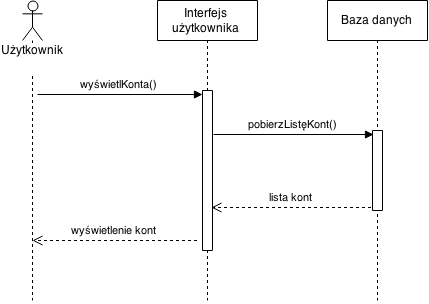
\includegraphics[width=0.7\textwidth]{images/sequence-diagram-accounts-view.png}
  \caption{Diagram sekwencji dla przypadku użycia~\ref{par:accountsView}~--~Wyświetlenie listy kont}
\end{figure}

\paragraph{Utworzenie nowego konta\newline}
\label{par:accountCreate}
Funkcja~specjalizująca~dla~\ref{par:accountsView}~--~Wyświetlanie listy kont.\\

\textit{Opis słowny} -- niniejszy przypadek użycia umożliwia użytkownikowi dodawanie nowych kont. Dzięki temu ma~on możliwość kontrolowania stanu wszystkich posiadanych przez niego fizycznie kont -- np. oszczędnościowych lub walutowych oraz definiowania transakcji pomiędzy nimi.\\

\begin{tabular}{|l|p{9cm}|}
  \hline \textbf{Aktor} & Użytkownik \\ \hline
  \textbf{Warunki początkowe} & Użytkownik jest zalogowany \\ \hline
  \textbf{Opis przebiegu interakcji} & Wybór strony z~kontami, kliknięcie przycisku, wprowadzenie danych oraz zatwierdzenie \\ \hline
  \textbf{Sytuacje wyjątkowe} & Niepoprawne dane \\ \hline
  \textbf{Warunki końcowe} & Nowe konto dodane do systemu \\ \hline
\end{tabular}\\\\

\noindent \textit{Scenariusz główny:}
\begin{enumerate}
  \item[1-3.] Jak w~funkcji generalizującej~\ref{par:accountsView}~--~Wyświetlanie listy kont.
  \item[4.] Użytkownik klika przycisk ,,Dodaj nowe konto''.
  \item[5.] Aplikacja wyświetla okno zawierające pola z~danymi dla nowego konta.
  \item[6.] Użytkownik wprowadza nazwę konta, początkowe saldo, wybiera walutę, typ konta i~klika przycisk ,,Dodaj''.
  \item[7.] System weryfikuje wprowadzone dane (np. czy para użytkownik-nazwa jest unikatowa).
  \item[8.] Jeśli dane są~prawidłowe, system tworzy nowe konto i~powiadamia o~tym użytkownika.
\end{enumerate}

\noindent \textit{Scenariusz alternatywny -- niepoprawne dane:}
\begin{enumerate}
  \item[1-7.] Jak w~scenariuszu głównym.
  \item[8.] System wyświetla informację o wykrytym błędzie.
  \item[9.] Użytkownik poprawia dane i~wciska przycisk ,,Dodaj''.
  \item[10.] Powrót do kroku 7 ze~scenariusza głównego.
\end{enumerate}

\begin{figure}[H]
  \centering
  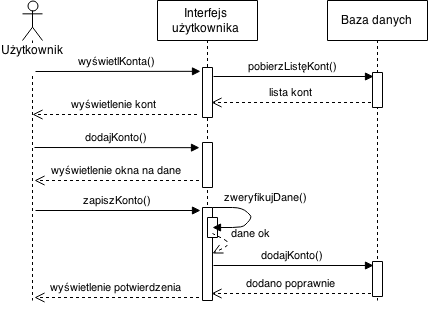
\includegraphics[width=0.7\textwidth]{images/sequence-diagram-account-create.png}
  \caption{Diagram sekwencji dla przypadku użycia~\ref{par:accountCreate}~--~Utworzenie nowego konta}
\end{figure}

\paragraph{Edycja danych konta\newline}
\label{par:accountEdit}
Funkcja~specjalizująca~dla~\ref{par:accountsView}~--~Wyświetlanie listy kont.\\

\textit{Opis słowny} -- niniejszy przypadek użycia umożliwia użytkownikowi edycję danych konta. Dzięki temu ma~on możliwość aktualizowania danych oraz zapewnienia ich zgodności ze~stanem faktycznym -- poza systemem.\\

\begin{tabular}{|l|p{9cm}|}
  \hline \textbf{Aktor} & Użytkownik \\ \hline
  \textbf{Warunki początkowe} & Użytkownik jest zalogowany i~posiada przynajmniej jedno konto \\ \hline
  \textbf{Opis przebiegu interakcji} & Wybór strony z~kontami, wybór konta, kliknięcie przycisku, wprowadzenie danych oraz zatwierdzenie \\ \hline
  \textbf{Sytuacje wyjątkowe} & Niepoprawne dane \\ \hline
  \textbf{Warunki końcowe} & Edycja danych konta w~systemie \\ \hline
\end{tabular}\\\\

\noindent \textit{Scenariusz główny:}
\begin{enumerate}
  \item[1-3.] Jak w~funkcji generalizującej~\ref{par:accountsView}~--~Wyświetlanie listy kont.
  \item[4.] Użytkownik zaznacza jedno z~kont i~klika przycisk ,,Edytuj'' obok niego.
  \item[5.] Aplikacja wyświetla okno zawierające dane zaznaczonego konta.
  \item[6.] Użytkownik edytuje nazwę konta, walutę lub typ konta i~klika przycisk ,,Zapisz''.
  \item[7.] System weryfikuje wprowadzone dane (np. czy para użytkownik-nazwa jest unikatowa).
  \item[8.] Jeśli dane są~prawidłowe, system edytuje konto i~powiadamia o~tym użytkownika.
\end{enumerate}

\noindent \textit{Scenariusz alternatywny -- niepoprawne dane:}
\begin{enumerate}
  \item[1-7.] Jak w~scenariuszu głównym.
  \item[8.] System wyświetla informację o wykrytym błędzie.
  \item[9.] Użytkownik poprawia dane i~wciska przycisk ,,Zapisz''.
  \item[10.] Powrót do kroku 7 ze~scenariusza głównego.
\end{enumerate}

\begin{figure}[H]
  \centering
  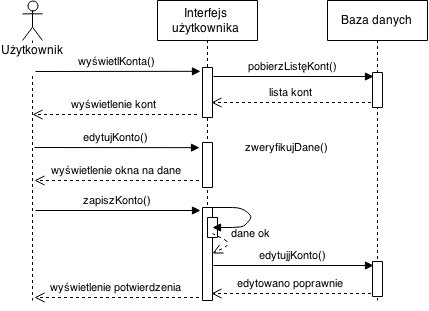
\includegraphics[width=0.7\textwidth]{images/sequence-diagram-account-edit.png}
  \caption{Diagram sekwencji dla przypadku użycia~\ref{par:accountEdit}~--~Edycja danych konta}
\end{figure}

\paragraph{Usunięcie konta\newline}
\label{par:accountDelete}
Funkcja~specjalizująca~dla~\ref{par:accountsView}~--~Wyświetlanie listy kont.\\

\textit{Opis słowny} -- niniejszy przypadek użycia umożliwia użytkownikowi usunięcie konta. Dzięki temu ma~on możliwość ukrycia w~systemie kont już nieużywanych lub nieaktywnych.\\

\begin{tabular}{|l|p{9cm}|}
  \hline \textbf{Aktor} & Użytkownik \\ \hline
  \textbf{Warunki początkowe} & Użytkownik jest zalogowany i~posiada przynajmniej jedno konto \\ \hline
  \textbf{Opis przebiegu interakcji} & Wybór strony z~kontami, wybór konta, kliknięcie przycisku oraz zatwierdzenie \\ \hline
  \textbf{Sytuacje wyjątkowe} & Anulowanie akcji \\ \hline
  \textbf{Warunki końcowe} & Usunięcie konta z~systemu \\ \hline
\end{tabular}\\\\

\noindent \textit{Scenariusz główny:}
\begin{enumerate}
  \item[1-3.] Jak w~funkcji generalizującej~\ref{par:accountsView}~--~Wyświetlanie listy kont.
  \item[4.] Użytkownik zaznacza jedno z~kont i~klika przycisk ,,Usuń'' obok niego.
  \item[5.] Aplikacja wyświetla okno potwierdzenia.
  \item[6.] Użytkownik klika przycisk ,,Usuń'' w~wyświetlonym oknie.
  \item[7.] Aplikacja zamyka okno, usuwa konto i~odświeża listę kont.
\end{enumerate}

\noindent \textit{Scenariusz alternatywny -- przerwanie operacji przez użytkownika:}
\begin{enumerate}
  \item[1-5.] Jak w~scenariuszu głównym.
  \item[6.] Użytkownik wciska przycisk ,,Anuluj''.
  \item[7.] Aplikacja zamyka okno.
\end{enumerate}

\begin{figure}[H]
  \centering
  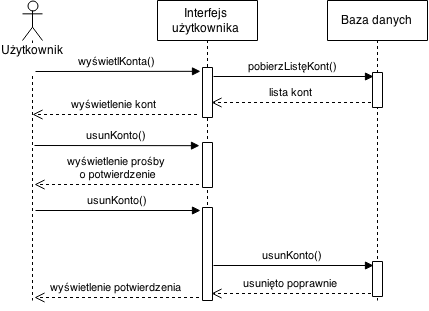
\includegraphics[width=0.7\textwidth]{images/sequence-diagram-account-delete.png}
  \caption{Diagram sekwencji dla przypadku użycia~\ref{par:accountDelete}~--~Usunięcie konta}
\end{figure}

\subsubsection{Opis przypadków użycia -- transakcje}

\begin{figure}[H]
  \centering
  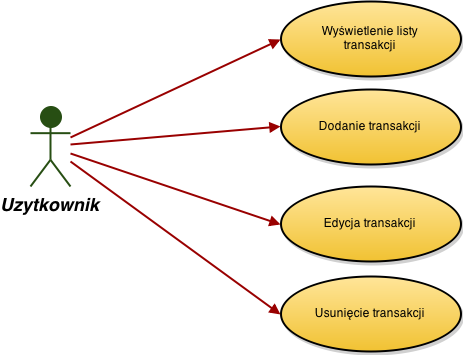
\includegraphics[width=0.9\textwidth]{images/transactions_use_cases.png}
  \caption{Diagram przypadków użycia związanych z~zarządzaniem transakcjami.}
\end{figure}

\paragraph{Wyświetlanie listy transakcji\newline}
\label{par:transactionsView}
Wykorzystuje~\ref{par:login}~--~Logowanie do~aplikacji.\\
\indent Funkcja generalizująca dla~\ref{par:transactionCreate},~\ref{par:transactionEdit} oraz~\ref{par:transactionDelete}.\\

\textit{Opis słowny} -- użytkownik będzie chciał wyświetlić listę transakcji zarejestrowanych w~systemie. Oprócz zwykłej listy zebranych danych, potrzebna jest możliwość filtrowania, co~ułatwi użytkownikowi przeglądanie listy.

\begin{longtable}{|p{5cm}|p{7cm}|}
  \hline \textbf{Aktor} & Użytkownik \\
  \hline \textbf{Warunki początkowe} & Użytkownik jest zalogowany \\
  \hline \textbf{Opis przebiegu interakcji} & Wybór strony z~transakcjami, wprowadzenie parametrów filtrowania \\
  \hline \textbf{Sytuacje wyjątkowe} & Żądanie filtrowania danych \\
  \hline \textbf{Warunki końcowe} & Wyświetlona lista żądanych transakcji \\
  \hline
\end{longtable}

\noindent \textit{Scenariusz główny:}
\begin{enumerate}
  \item Użytkownik otwiera stronę ,,Transakcje''.
  \item Jeśli użytkownik nie jest zalogowany, aplikacja wymaga zalogowania, inicjując~\ref{par:login}~--~Logowanie do~aplikacji.
  \item Aplikacja wyświetla listę transakcji powiązanych z~kontem danego użytkownika.
\end{enumerate}

\noindent \textit{Scenariusz alternatywny -- filtrowanie transakcji:}
\begin{enumerate}
  \item[1-3.] Jak w~scenariuszu głównym.
  \item[4.] Użytkownik wprowadza parametry filtrowania jak nazwa użytkownika, kategoria albo data transakcji.
  \item[5.] Aplikacja odświeża listę transakcji, wyświetlając tylko te, które pasują do podanych filtrów.
\end{enumerate}

\begin{figure}[H]
  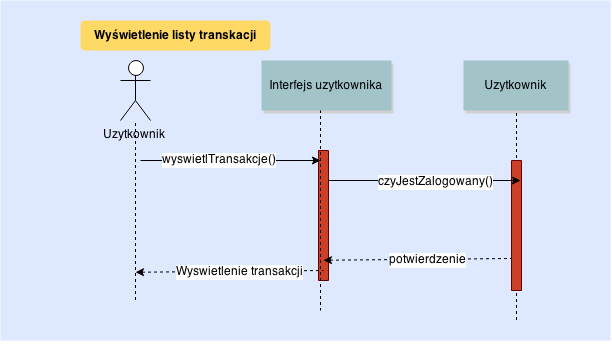
\includegraphics[width=\textwidth]{images/wyswietl_transakcje.png}
  \caption{Diagram sekwencji dla przypadku użycia~\ref{par:transactionsView}~--~Wyświetlenie listy transakcji (scenariusz główny)}
\end{figure}

\paragraph{Utworzenie nowej transakcji\newline}
\label{par:transactionCreate}
Funkcja~specjalizująca~dla~\ref{par:transactionsView}~--~Wyświetlanie listy transakcji.\\

\textit{Opis słowny} -- jedna z~podstawowych funkcjonalności systemu to~dodawanie transakcji, których koszty będą sumowane i~nadzorowane. Akcje te~mają miejsce, gdy użytkownik chce dodać wydatek do systemu.

\begin{longtable}{|p{5cm}|p{7cm}|}
  \hline \textbf{Aktor} & Użytkownik \\
  \hline \textbf{Warunki początkowe} & Użytkownik jest zalogowany oraz posiada przynajmniej jedno konto \\
  \hline \textbf{Opis przebiegu interakcji} & Wybór strony z~transakcjami i~wciśnięcie dodaj, uzupełnienie danych i~zapisanie \\
  \hline \textbf{Sytuacje wyjątkowe} & Wprowadzenie niepoprawnych danych \\
  \hline \textbf{Warunki końcowe} & Dodanie nowej transakcji \\
  \hline
\end{longtable}

\noindent \textit{Scenariusz główny:}
\begin{enumerate}
  \item[1-3.] Jak w~scenariuszu generalizującym~\ref{par:transactionsView}~--~Wyświetlenie listy transakcji.
  \item[4.] Użytkownik wciska przycisk ,,Dodaj transakcję''.
  \item[5.] Aplikacja wyświetla okno z~polami do~wprowadzania danych dotyczących transakcji.
  \item[6.] Użytkownik wprowadza rodzaj transakcji (wpływ/wydatek/transfer), konto od/do, wprowadza wartość, datę, opis i~klika przycisk ,,Dodaj''.
  \item[7.] System weryfikuje wprowadzone dane (np. czy na danym koncie znajduje się wystarczająca ilość pieniędzy).
  \item[8.] Jeśli dane są poprawne, system tworzy nową transakcję, przelicza ilość pieniędzy pozostałych na~koncie i~informuje użytkownika.
\end{enumerate}

\noindent \textit{Scenariusz alternatywny -- niepoprawne dane:}
\begin{enumerate}
  \item[1-7.] Jak w~scenariuszu głównym.
  \item[8.] System wyświetla informację o~wykrytym błędzie.
  \item[9.] Użytkownik poprawia dane i~wciska przycisk ,,Dodaj''.
  \item[10.] Powrót do kroku 7 ze~scenariusza głównego.
\end{enumerate}

\begin{figure}[H]
  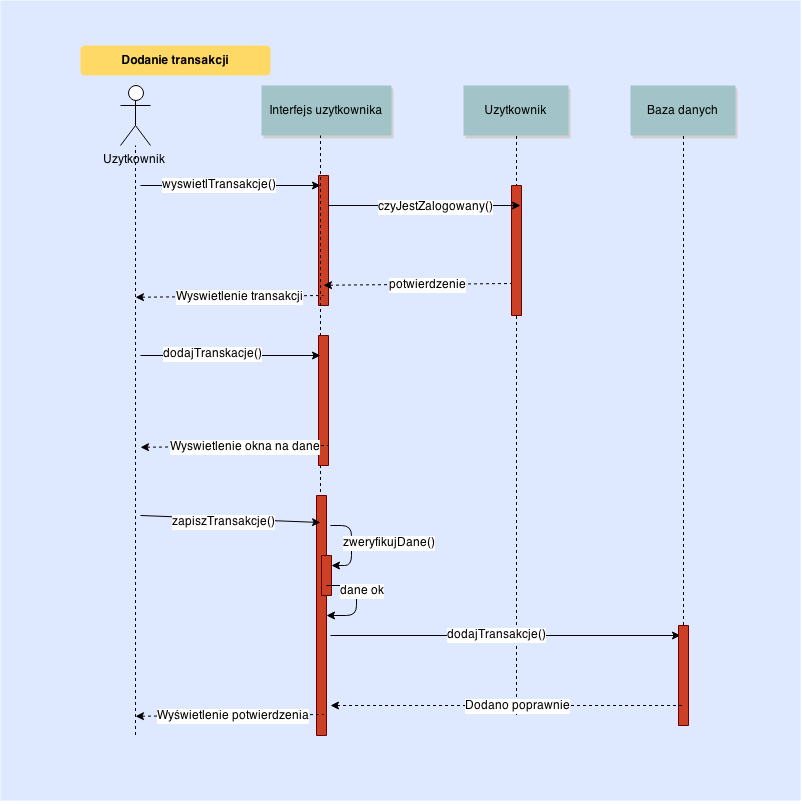
\includegraphics[width=\textwidth]{images/dodanie_transakcji.png}
  \caption{Diagram sekwencji dla przypadku użycia~\ref{par:transactionCreate}~--~Utworzenie nowej transakcji (scenariusz główny)}
\end{figure}

\paragraph{Edycja transakcji\newline}
\label{par:transactionEdit}
Funkcja~specjalizująca~dla~\ref{par:transactionsView}~--~Wyświetlanie listy transakcji.\\

\textit{Opis słowny} -- modyfikacja danych dotyczących wybranej transakcji może być przydatna w~sytuacji, gdy użytkownik wprowadzi błędne dane w~kontekście logicznym, ale które będą poprawnie w~sensie formalnym.

\begin{longtable}{|p{5cm}|p{7cm}|}
  \hline \textbf{Aktor} & Użytkownik \\
  \hline \textbf{Warunki początkowe} & Użytkownik jest zalogowany oraz istnieją transakcje w~systemie \\
  \hline \textbf{Opis przebiegu interakcji} & Wybór strony z transakcjami, wybór żądanej transakcji, modyfikacja danych i~zapisanie \\
  \hline \textbf{Sytuacje wyjątkowe} & Wprowadzenie niepoprawnych danych \\
  \hline \textbf{Warunki końcowe} & Dodanie nowej transakcji \\
  \hline
\end{longtable}

\noindent \textit{Scenariusz główny:}
\begin{enumerate}
  \item[1-3.] Jak w~scenariuszu generalizującym~\ref{par:transactionsView}~--~Wyświetlenie listy transakcji.
  \item[4.] Użytkownik wybiera jedną z~transakcji i~wciska przycisk ,,Edytuj''.
  \item[5.] Aplikacja wyświetla okno z~informacjami o~transakcji.
  \item[6.] Użytkownik modyfikuje dane transakcji (wpływ/wydatek/transfer), konto od/do, wprowadza wartość, datę, opis i~klika przycisk ,,Zapisz''.
  \item[7.] System weryfikuje wprowadzone dane (np. czy na danym koncie znajduje się wystarczająca ilość pieniędzy).
  \item[8.] Jeśli dane są~poprawne, system zapisuje transakcję, przelicza ilość pieniędzy pozostałych na~koncie i~informuje użytkownika.
\end{enumerate}

\noindent \textit{Scenariusz alternatywny -- niepoprawne dane:}
\begin{enumerate}
  \item[1-7.] Jak w~scenariuszu głównym.
  \item[8.] System wyświetla informację o~wykrytym błędzie i~czeka na~poprawkę.
  \item[9.] Użytkownik poprawia dane i~wciska przycisk ,,Zapisz''.
  \item[10.] Powrót do~kroku 7 ze~scenariusza głównego.
\end{enumerate}

\begin{figure}[H]
  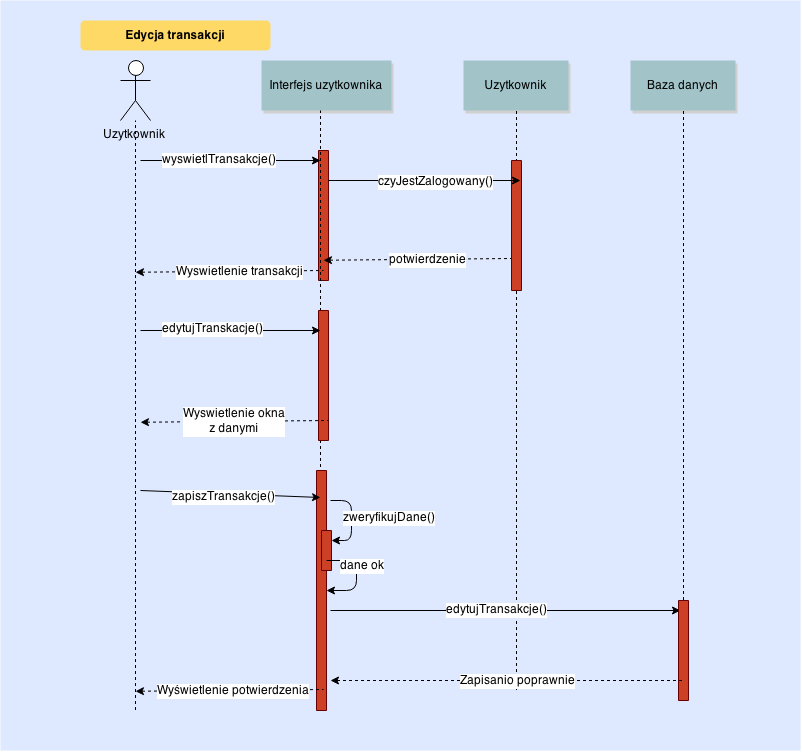
\includegraphics[width=\textwidth]{images/edycja_transakcji.png}
  \caption{Diagram sekwencji dla przypadku użycia~\ref{par:transactionEdit}~--~Edycja transakcji (scenariusz główny)}
\end{figure}

\paragraph{Usuwanie transakcji\newline}
\label{par:transactionDelete}
Funkcja~specjalizująca~dla~\ref{par:transactionsView}~--~Wyświetlanie listy transakcji.\\

\textit{Opis słowny} -- akcje opisane poniżej mają miejsce w~przypadku gdy np. użytkownik zwrócił towar którego dotyczyła transakcja, którą już wprowadził.

\begin{longtable}{|p{5cm}|p{7cm}|}
  \hline \textbf{Aktor} & Użytkownik \\
  \hline \textbf{Warunki początkowe} & Użytkownik jest zalogowany oraz istnieją transakcje w~systemie \\
  \hline \textbf{Opis przebiegu interakcji} & Wybór strony z transakcjami, wybór żądanej transakcji, usunięcie jej \\
  \hline \textbf{Sytuacje wyjątkowe} & Brak \\
  \hline \textbf{Warunki końcowe} & Usunięcie transakcji \\
  \hline
\end{longtable}

\noindent \textit{Scenariusz główny:}
\begin{enumerate}
  \item[1-3.] Jak w~scenariuszu generalizującym~\ref{par:transactionsView}~--~Wyświetlenie listy transakcji.
  \item[4.] Użytkownik wybiera jedną z~transakcji i~wciska przycisk ,,Usuń''.
  \item[5.] Aplikacja wyświetla okienko wymagające potwierdzenia operacji.
  \item[6.] Użytkownik potwierdza operację wciskając przycisk ,,Usuń''.
  \item[7.] Aplikacja zamyka okienko, usuwa transakcję, przelicza ilość pieniędzy na koncie i odświeża listę transakcji.
\end{enumerate}

\noindent \textit{Scenariusz alternatywny -- przerwanie operacji przez użytkownika:}
\begin{enumerate}
  \item[1-5.] Jak w~scenariuszu głównym.
  \item[6.] Użytkownik wciska przycisk ,,Anuluj''.
  \item[7.] Aplikacja zamyka okno.
\end{enumerate}

\begin{figure}[H]
  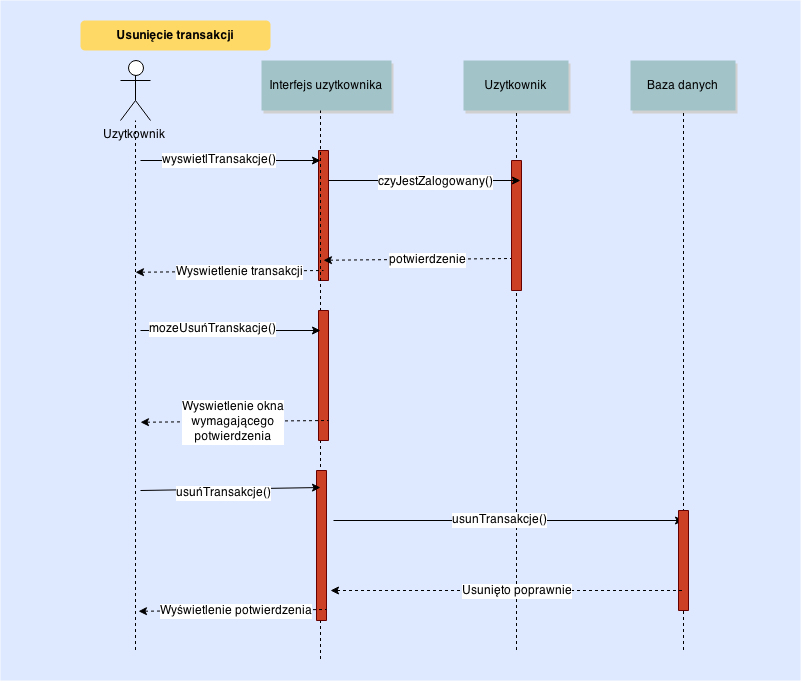
\includegraphics[width=\textwidth]{images/usun_transakcje.png}
  \caption{Diagram sekwencji dla przypadku użycia~\ref{par:transactionDelete}~--~Usuwanie transakcji (scenariusz główny)}
\end{figure}

\subsubsection{Opis przypadków użycia -- budżet}

\begin{figure}[H]
  \centering
  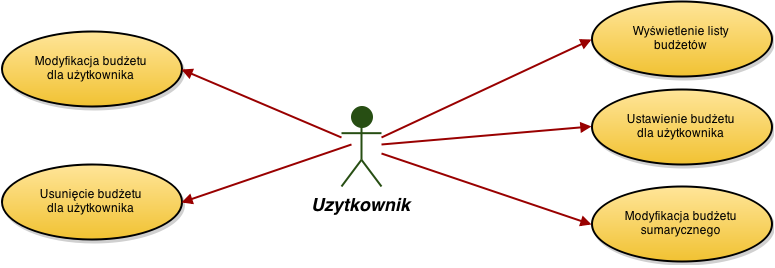
\includegraphics[width=0.9\textwidth]{images/budgets_use_cases.png}
  \caption{Diagram przypadków użycia związanych z~zarządzaniem budżetami.}
\end{figure}

\paragraph{Wyświetlenie budżetów ustawionych w systemie\newline}
\label{par:budgetsList}
Wykorzystuje~\ref{par:login}~--~Logowanie do~aplikacji.\\
\indent Funkcja generalizująca dla~\ref{par:userBudget},~\ref{par:usersBudget},~\ref{par:userBudgetEdit} oraz~\ref{par:userBudgetDelete}.\\

\textit{Opis słowny} -- głównym zadaniem systemu jest nadzorowanie domowego budżetu. Użytkownik będzie chciał przejrzeć aktualny stan budżetów sumarycznych oraz poszczególnych dla każdego z~zarejestrowanych użytkowników.

\begin{longtable}{|p{5cm}|p{7cm}|}
  \hline \textbf{Aktor} & Użytkownik \\
  \hline \textbf{Warunki początkowe} & Użytkownik jest zalogowany \\
  \hline \textbf{Opis przebiegu interakcji} & Wybór strony z budżetami \\
  \hline \textbf{Sytuacje wyjątkowe} & Żądanie filtrowania danych \\
  \hline \textbf{Warunki końcowe} & Wyświetlenie żądanych budżetów \\
  \hline
\end{longtable}

\noindent \textit{Scenariusz główny:}
\begin{enumerate}
  \item Użytkownik otwiera stronę ,,Budżety''.
  \item Jeśli użytkownik nie jest zalogowany, aplikacja wymaga zalogowania, inicjując~\ref{par:login}~--~Logowanie do~aplikacji.
  \item Aplikacja wyświetla budżet sumaryczny dla wszystkich użytkowników oraz listę użytkowników z~budżetami dla każdego z~nich.
\end{enumerate}

\noindent \textit{Scenariusz alternatywny -- filtrowanie wyników:}
\begin{enumerate}
  \item[1-3.] Jak w~scenariuszu głównym.
  \item[4.] Użytkownik wprowadza nazwę konta, którego budżet ma~zostać wyświetlony i~wciska ,,Enter''.
  \item[5.] Aplikacja odświeża listę budżetów wyświetlając tylko jeden dla podanego użytkownika.
\end{enumerate}

\paragraph{Ustawienie budżetu dla określonego użytkownika\newline}
\label{par:userBudget}
Funkcja~specjalizująca~dla~\ref{par:budgetsList}~--~Wyświetlanie budżetów.\\

\textit{Opis słowny} -- celem lepszej kontroli wydatków, użytkownik może chcieć ustawić limit budżetu dla określonego użytkownika, aby ten nie mógł przekroczyć określonej kwoty.

\begin{longtable}{|p{5cm}|p{7cm}|}
  \hline \textbf{Aktor} & Użytkownik \\
  \hline \textbf{Warunki początkowe} & Użytkownik jest zalogowany \\
  \hline \textbf{Opis przebiegu interakcji} & Wybór strony z budżetami, wprowadzenie wymaganych danych, zapisanie nowego budżetu \\
  \hline \textbf{Sytuacje wyjątkowe} & Błędne wprowadzenie danych, przerwanie operacji \\
  \hline \textbf{Warunki końcowe} & Dodanie nowego limitu dla użytkownika \\
  \hline
\end{longtable}

\noindent \textit{Scenariusz główny:}
\begin{enumerate}
  \item[1-3.] Jak w~scenariuszu generalizującym~\ref{par:budgetsList}~--~Wyświetlenie budżetów występujących w~systemie.
  \item[4.] Użytkownik wciska przycisk ,,Dodaj''.
  \item[5.] Aplikacja wyświetla okno z możliwością wyboru konta i~wprowadzenia nowego budżetu.
  \item[6.] Użytkownik wybiera konto, wprowadza nowy budżet i~wciska przycisk "Dodaj".
  \item[7.] Aplikacja weryfikuje poprawność wprowadzonych danych (np. czy liczba nie jest ujemna).
  \item[8.] Jeśli wartość jest poprawna system zapisuje nową wartość budżetu, zamyka okno i~aktualizuje stronę z~budżetami.
\end{enumerate}

\noindent \textit{Scenariusz alternatywny -- przerwanie operacji przez użytkownika:}
\begin{enumerate}
  \item[1-5.] Jak w~scenariuszu głównym.
  \item[6.] Użytkownik wciska przycisk "Anuluj".
  \item[7.] Aplikacja zamyka okno.
\end{enumerate}

\noindent \textit{Scenariusz alternatywny -- niepoprawne dane:}
\begin{enumerate}
  \item[1-7.] Jak w~scenariuszu głównym.
  \item[8.] System wyświetla informację o~niepoprawnych danych.
  \item[9.] Użytkownik wprowadza nową wartość i~wciska przycisk ,,Dodaj''.
  \item[10.] Powrót do kroku 7 ze~scenariusza głównego.
\end{enumerate}

\begin{figure}[H]
  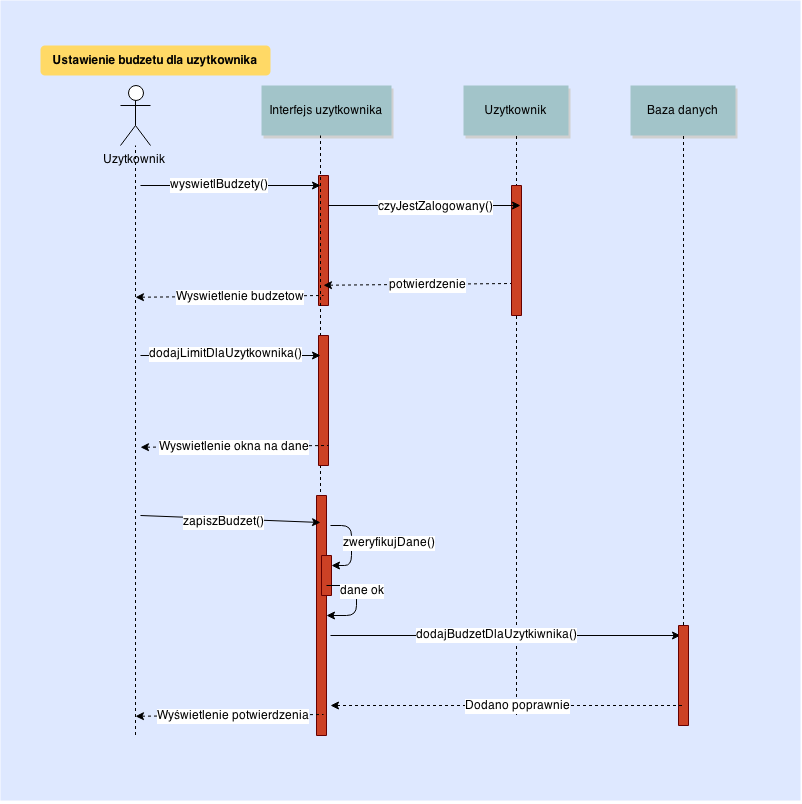
\includegraphics[width=\textwidth]{images/dodanie_budzetu_dla_usera.png}
  \caption{Diagram sekwencji dla przypadku użycia~\ref{par:userBudget}~--~Ustawienie budżetu dla określonego użytkownika (scenariusz główny)}
\end{figure}

\paragraph{Modyfikacja budżetu sumarycznego dla wszystkich użytkowników\newline}
\label{par:usersBudget}
Funkcja~specjalizująca~dla~\ref{par:budgetsList}~--~Wyświetlanie budżetów.\\

\textit{Opis słowny} -- oprócz ustawiania limitu miesięcznego dla danego użytkownika, kluczowym elementem systemu jest modyfikacja limitu sumarycznego dla wszystkich użytkowników danej aplikacji. Wartość ta~musi być zawsze ustawiona, lecz użytkownik może ją~dowolnie modyfikować.

\begin{longtable}{|p{5cm}|p{7cm}|}
  \hline \textbf{Aktor} & Użytkownik \\
  \hline \textbf{Warunki początkowe} & Użytkownik jest zalogowany \\
  \hline \textbf{Opis przebiegu interakcji} & Wybór strony z budżetami, wprowadzenie wymaganych danych, zapisanie budżetu \\
  \hline \textbf{Sytuacje wyjątkowe} & Błędne wprowadzenie danych, przerwanie operacji \\
  \hline \textbf{Warunki końcowe} & Zmodyfikowanie budżetu sumarycznego \\
  \hline
\end{longtable}

\noindent \textit{Scenariusz główny:}
\begin{enumerate}
  \item[1-3.] Jak w~scenariuszu generalizującym~\ref{par:budgetsList}~--~Wyświetlenie budżetów występujących w~systemie.
  \item[4.] Użytkownik wciska przycisk "Edytuj" obok pola wyświetlającego budżet sumaryczny.
  \item[5.] Aplikacja wyświetla okno z~możliwością wprowadzenia nowego budżetu sumarycznego.
  \item[6.] Użytkownik wprowadza nowy budżet i~wciska przycisk ,,Zapisz''.
  \item[7.] Aplikacja weryfikuje poprawność wprowadzonych danych (np. czy liczba nie jest ujemna).
  \item[8.] Jeśli wartość jest poprawna, system zapisuje nową wartość budżetu, zamyka okno i~aktualizuje stronę z budżetami.
\end{enumerate}

\noindent \textit{Scenariusz alternatywny -- przerwanie operacji przez użytkownika:}
\begin{enumerate}
  \item[1-5.] Jak w~scenariuszu głównym.
  \item[6.] Użytkownik wciska przycisk "Anuluj".
  \item[7.] Aplikacja zamyka okno.
\end{enumerate}

\noindent \textit{Scenariusz alternatywny -- niepoprawne dane:}
\begin{enumerate}
  \item[1-7.] Jak w~scenariuszu głównym.
  \item[8.] System wyświetla informację o~niepoprawnych danych.
  \item[9.] Użytkownik wprowadza nową wartość i~wciska przycisk ,,Zapisz''.
  \item[10.] Powrót do kroku 7 ze~scenariusza głównego.
\end{enumerate}

\begin{figure}[H]
  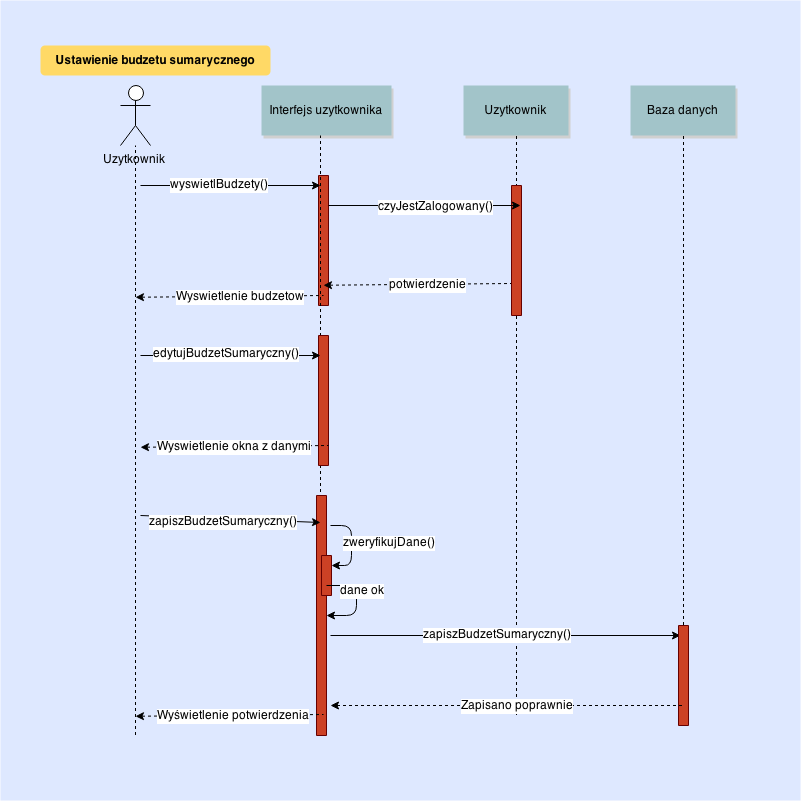
\includegraphics[width=\textwidth]{images/modyfikacja_budzetu_sumarycznego.png}
  \caption{Diagram sekwencji dla przypadku użycia~\ref{par:usersBudget}~--~Ustawienie budżetu sumarycznego (scenariusz główny)}
\end{figure}

\paragraph{Modyfikacja budżetu dla określonego użytkownika\newline}
\label{par:userBudgetEdit}
Funkcja~specjalizująca~dla~\ref{par:budgetsList}~--~Wyświetlanie budżetów.\\

\textit{Opis słowny} -- system musi pozwolić również modyfikować wcześniej ustawiony budżet dla poszczególnych użytkowników, gdyż limity te~mogą się zmieniać np. gdy dziecko dostanie większe kieszonkowe.

\begin{longtable}{|p{5cm}|p{7cm}|}
  \hline \textbf{Aktor} & Użytkownik \\
  \hline \textbf{Warunki początkowe} & Użytkownik jest zalogowany \\
  \hline \textbf{Opis przebiegu interakcji} & Wybór strony z budżetami, wprowadzenie wymaganych danych, zapisanie budżetu \\
  \hline \textbf{Sytuacje wyjątkowe} & Błędne wprowadzenie danych, przerwanie operacji \\
  \hline \textbf{Warunki końcowe} & Zmodyfikowanie budżetu użytkownika \\
  \hline
\end{longtable}

\noindent \textit{Scenariusz główny:}
\begin{enumerate}
  \item[1-3.] Jak w~scenariuszu generalizującym~\ref{par:budgetsList}~--~Wyświetlenie budżetów występujących w~systemie.
  \item[4.] Użytkownik wciska przycisk ,,Edytuj'' obok pola wyświetlającego budżet dla określonego użytkownika.
  \item[5.] Aplikacja wyświetla okno z~możliwością wprowadzenia nowego budżetu.
  \item[6.] Użytkownik wprowadza nowy budżet i~wciska przycisk ,,Zapisz''.
  \item[7.] Aplikacja weryfikuje poprawność wprowadzonych danych (np. czy liczba nie jest ujemna).
  \item[8.] Jeśli wartość jest poprawna, system zapisuje nową wartość budżetu, zamyka okno i~aktualizuje stronę z~budżetami.
\end{enumerate}

\noindent \textit{Scenariusz alternatywny -- przerwanie operacji przez użytkownika:}
\begin{enumerate}
  \item[1-5.] Jak w~scenariuszu głównym.
  \item[6.] Użytkownik wciska przycisk ,,Anuluj''.
  \item[7.] Aplikacja zamyka okno.
\end{enumerate}

\noindent \textit{Scenariusz alternatywny -- niepoprawne dane:}
\begin{enumerate}
  \item[1-7.] Jak w~scenariuszu głównym.
  \item[8.] System wyświetla informację o~niepoprawnych danych.
  \item[9.] Użytkownik wprowadza nową wartość i~wciska przycisk ,,Zapisz''.
  \item[10.] Powrót do kroku 7 ze~scenariusza głównego.
\end{enumerate}

\begin{figure}[H]
  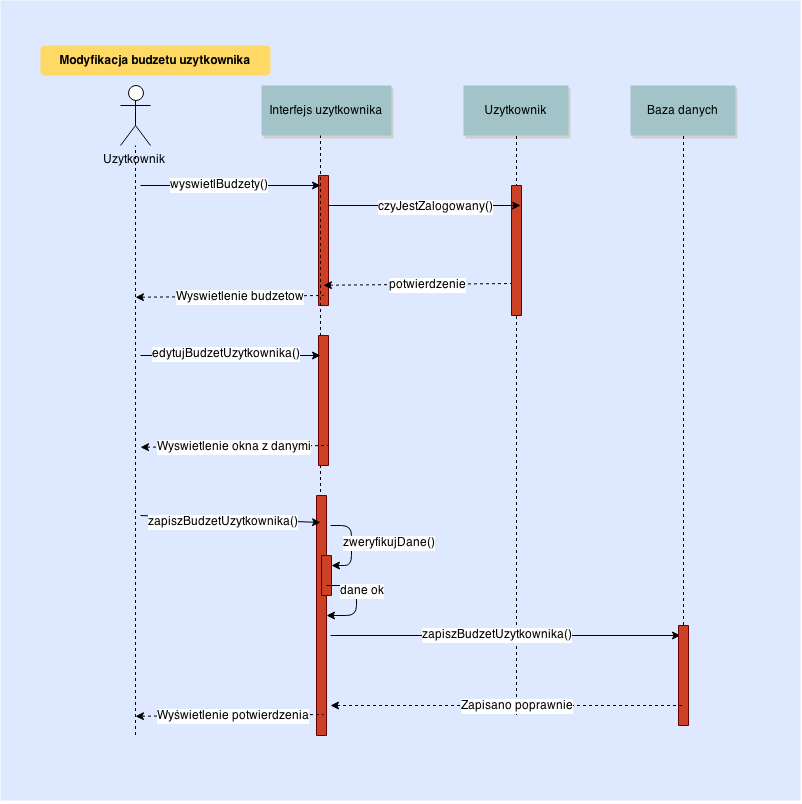
\includegraphics[width=\textwidth]{images/modyfikacja_budzetu_uzytkownika.png}
  \caption{Diagram sekwencji dla przypadku użycia~\ref{par:userBudgetEdit}~--~Modyfikacja budżetu dla określonego użytkownika (scenariusz główny)}
\end{figure}

\paragraph{Usunięcie budżetu dla określonego użytkownika\newline}
\label{par:userBudgetDelete}
Funkcja~specjalizująca~dla~\ref{par:budgetsList}~--~Wyświetlanie budżetów.\\

\textit{Opis słowny} -- akcje te~będą wykonane, gdy np. użytkownik nie będzie dłużej korzystał z~podanej aplikacji lub limit miesięczny przestał go~dotyczyć. Poza tym, polityka ustalania budżetów może ulec zmianie -- na~przykład zamiast ustawiania budżetów na~poszczególne osoby, zacznie obowiązywać tylko budżet sumaryczny.

\begin{longtable}{|p{5cm}|p{7cm}|}
  \hline \textbf{Aktor} & Użytkownik \\
  \hline \textbf{Warunki początkowe} & Użytkownik jest zalogowany oraz istnieje limit ustawiony na~użytkownika \\
  \hline \textbf{Opis przebiegu interakcji} & Wybór strony z budżetami, usunięcie wybranego budżetu \\
  \hline \textbf{Sytuacje wyjątkowe} & Przerwanie operacji \\
  \hline \textbf{Warunki końcowe} & Usunięcie budżetu użytkownika \\
  \hline
\end{longtable}

\noindent \textit{Scenariusz główny:}
\begin{enumerate}
  \item[1-3.] Jak w~scenariuszu generalizującym~\ref{par:budgetsList}~--~Wyświetlenie budżetów występujących w~systemie.
  \item[4.] Użytkownik wciska przycisk ,,Usuń'' obok pola wyświetlającego budżet dla określonego użytkownika.
  \item[5.] Aplikacja wyświetla okno wymagające potwierdzenia operacji.
  \item[6.] Użytkownik potwierdza operację wciskając przycisk ,,Usuń''.
  \item[7.] System usuwa budżet dla określonego użytkownika, zamyka okno i~odświeża stronę z~budżetami.
\end{enumerate}

\noindent \textit{Scenariusz alternatywny -- przerwanie operacji przez użytkownika:}
\begin{enumerate}
  \item[1-5.] Jak w~scenariuszu głównym.
  \item[6.] Użytkownik klika przycisk ,,Anuluj''.
  \item[7.] Aplikacja zamyka okno.
\end{enumerate}

\begin{figure}[H]
  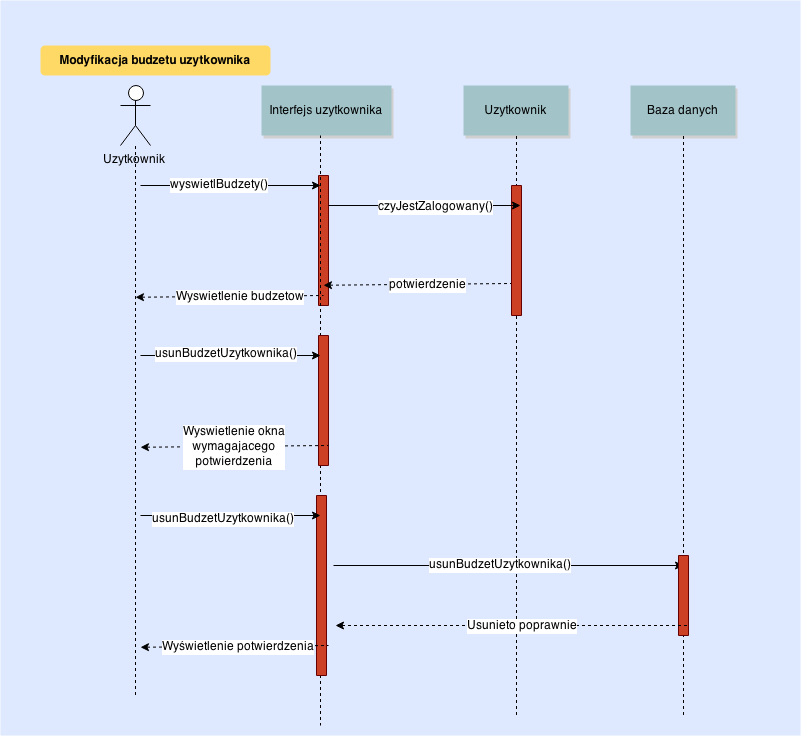
\includegraphics[width=\textwidth]{images/usun_budzet_uzytkownika.png}
  \caption{Diagram sekwencji dla przypadku użycia~\ref{par:userBudgetDelete}~--~Usunięcie budżetu dla określonego użytkownika (scenariusz główny)}
\end{figure}

\subsubsection{Opis przypadków użycia -- raporty}

% TODO diagram przypadków użycia - Kombajn

\paragraph{Konfiguracja raportu\newline}
\label{par:reportConfig}
Wykorzystuje~\ref{par:login}~--~Logowanie do~aplikacji.\\
\indent Funkcja generalizująca dla~\ref{par:reportView} oraz~\ref{par:reportExport}.\\

\textit{Opis słowny} -- istotną funkcją systemu jest generowanie raportów wizualizujących dane zebrane w~bazie. Użytkownik powinien mieć możliwość określenia budżetów i~zakresu transakcji, których raport ma~dotyczyć.

\begin{longtable}{|p{5cm}|p{7cm}|}
  \hline \textbf{Aktor} & Użytkownik \\
  \hline \textbf{Warunki początkowe} & Użytkownik jest zalogowany \\
  \hline \textbf{Opis przebiegu interakcji} & Wybór opcji raportu \\
  \hline \textbf{Sytuacje wyjątkowe} & Brak \\
  \hline \textbf{Warunki końcowe} & Brak \\
  \hline
\end{longtable}

\noindent \textit{Scenariusz główny:}
\begin{enumerate}
  \item Użytkownik otwiera stronę ,,Raport''.
  \item Jeśli użytkownik nie jest zalogowany, aplikacja wymaga zalogowania, inicjując~\ref{par:login}~--~Logowanie do~aplikacji.
  \item Aplikacja wyświetla pola~do wprowadzania opcji raportu
  \item Użytkownika wprowadza parametry raportu, takie jak zakres uwzględnionych transakcji (budżet sumaryczny/budżet indywidualny/wszystkie transakcje użytkownika), zakres dat, rodzaj raportu (tabela/wykres).
\end{enumerate}

\begin{figure}[H]
  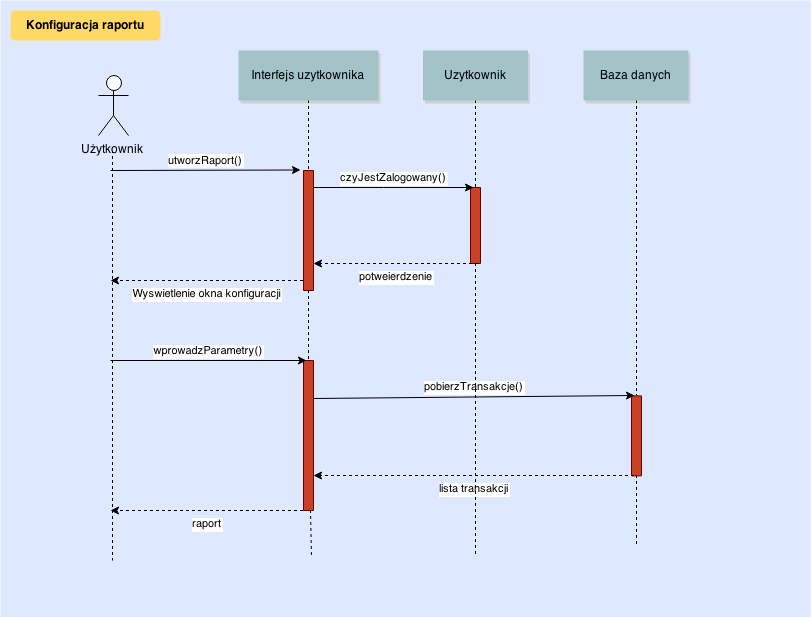
\includegraphics[width=\textwidth]{images/raport_konfig.png}
  \caption{Diagram sekwencji dla przypadku użycia~\ref{par:reportConfig}~--~Konfiguracja raportu (scenariusz główny)}
\end{figure}

\paragraph{Wyświetlanie raportu\newline}
\label{par:reportView}
\indent Funkcja specjalizująca dla~\ref{par:reportConfig}~--~Wyświetlanie konfiguracji raportu.\\

\textit{Opis słowny} -- użytkownik powinien mieć możliwość wyświetlenia raportu w~oknie aplikacji.

\begin{longtable}{|p{5cm}|p{7cm}|}
  \hline \textbf{Aktor} & Użytkownik \\
  \hline \textbf{Warunki początkowe} & Użytkownik jest zalogowany, parametry raportu są~wybrane \\
  \hline \textbf{Opis przebiegu interakcji} & Wyświetlenie raportu \\
  \hline \textbf{Sytuacje wyjątkowe} & Pusty raport \\
  \hline \textbf{Warunki końcowe} & Brak \\
  \hline
\end{longtable}

\noindent \textit{Scenariusz główny:}
\begin{enumerate}
  \item[1-4.] Jak w~scenariuszu generalizującym~\ref{par:reportConfig}~--~Wyświetlanie konfiguracji raportu.
  \item[5.] Użytkownik wciska przycisk ,,Wyświetl raport''.
  \item[6.] Aplikacja wyświetla okno z~raportem w~formie zgodnej z~konfiguracją.
  \item[7.] Użytkownik wciska przycisk ,,Zamknij''.
  \item[8.] Aplikacja zamyka okno.
\end{enumerate}

\noindent \textit{Scenariusz alternatywny~--~brak transakcji w raporcie}
\begin{enumerate}
  \item[1-5.] Jak w~scenariuszu głównym.
  \item[6.] Aplikacja wyświetla informację o~pustym raporcie.
  \item[7.] Powrót do kroku 1. scenariusza głównego.
\end{enumerate}

\begin{figure}[H]
  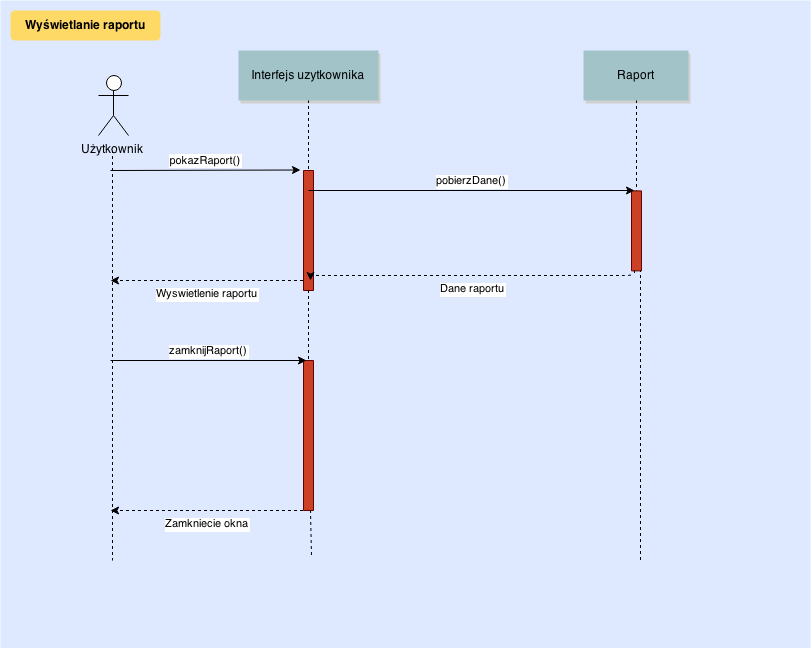
\includegraphics[width=\textwidth]{images/raport_show.png}
  \caption{Diagram sekwencji dla przypadku użycia~\ref{par:reportView}~--~Wyświetlanie raportu (scenariusz główny)}
\end{figure}

\paragraph{Zapisywanie raportu do pliku\newline}
\label{par:reportExport}
\indent Funkcja specjalizująca dla~\ref{par:reportConfig}~--~Wyświetlanie konfiguracji raportu.\\

\textit{Opis słowny} -- aplikacja powinna umożliwiać również zapisanie raportu do~pliku o~określonym formacie.

\begin{longtable}{|p{5cm}|p{7cm}|}
  \hline \textbf{Aktor} & Użytkownik \\
  \hline \textbf{Warunki początkowe} & Użytkownik jest zalogowany, parametry raportu są~wybrane \\
  \hline \textbf{Opis przebiegu interakcji} & Wybór katalogu i~nazwy pliku, zapis raportu \\
  \hline \textbf{Sytuacje wyjątkowe} & Pusty raport, przerwanie operacji \\
  \hline \textbf{Warunki końcowe} & Raport zapisany do pliku \\
  \hline
\end{longtable}

\noindent \noindent \textit{Scenariusz główny:}
\begin{enumerate}
  \item[1-4.] Jak w~scenariuszu generalizującym~\ref{par:reportConfig}~--~Wyświetlanie konfiguracji raportu.
  \item[5.] Użytkownik wciska przycisk ,,Zapisz raport''.
  \item[6.] Aplikacja wyświetla okno wyboru katalogu i~nazwy pliku.
  \item[7.] Użytkownik wybiera katalog i~nazwę pliku i~wciska przycisk ,,Zapisz''.
  \item[8.] Aplikacja zapisuje raport w~odpowiednim formacie do wybranego pliku i~zamyka okno.
\end{enumerate}

\noindent \textit{Scenariusz alternatywny~--~brak transakcji w raporcie}
\begin{enumerate}
  \item[1-5.] Jak w~scenariuszu głównym.
  \item[6.] Aplikacja wyświetla informację o~pustym raporcie.
  \item[7.] Powrót do kroku 1. scenariusza głównego.
\end{enumerate}

\noindent \textit{Scenariusz alternatywny~--~przerwanie operacji przez użytkownika}
\begin{enumerate}
  \item[1-6.] Jak w~scenariuszu głównym.
  \item[7.] Użytkownik wciska przycisk ,,Anuluj''.
  \item[8.] Aplikacja zamyka okno.
  \item[9.] Powrót do kroku 2. ze scenariusza głównego.
\end{enumerate}

\begin{figure}[H]
  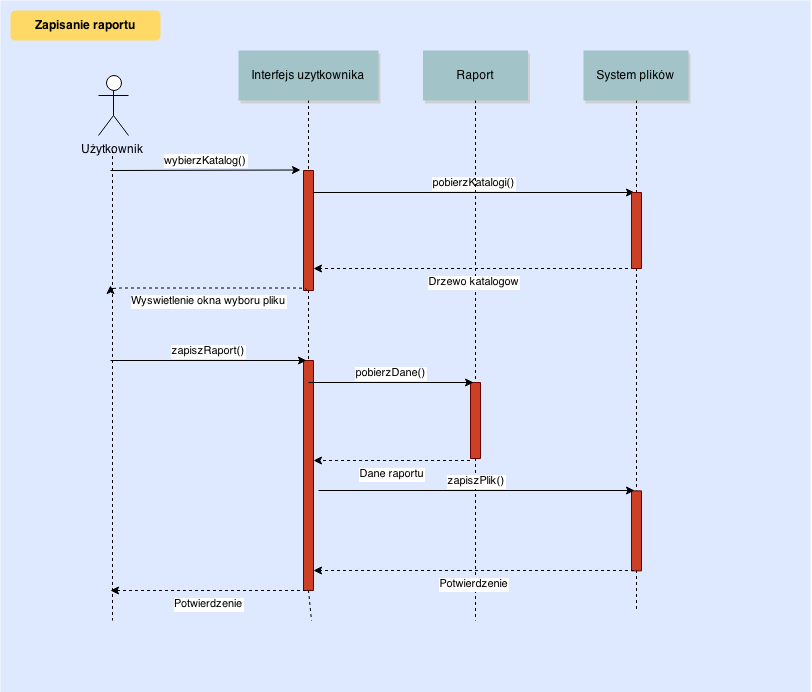
\includegraphics[width=\textwidth]{images/raport_export.png}
  \caption{Diagram sekwencji dla przypadku użycia~\ref{par:reportExport}~--~Zapisywanie raportu do pliku (scenariusz główny)}
\end{figure}

\newpage
\subsection{Wymagania niefunkcjonalne}

\subsubsection{Bezpieczeństwo}

\paragraph{Ograniczenia dostępu\newline}
Aplikacja nie może pozwalać niezalogowanym użytkownikom na dostęp do danych. Użytkownicy zalogowani mogą mieć dostęp wyłącznie do transakcji własnych oraz transakcji w~budżetach zbiorczych. Ponadto użytkownicy mają możliwość edycji wyłącznie własnych transakcji.

\paragraph{Zabezpieczenie przed nieautoryzowanym odczytem danych\newline}
Wszelkie dane przechowywane przez aplikację muszą być zabezpieczone przed odczytem i~modyfikacją bez pośrednictwa aplikacji. Dane nie powinny być przechowywane w~formacie jawnym.

\paragraph{Transakcyjność\newline}
Aplikacja nie może pozwalać na realizację niekompletnych operacji. W~wypadku wystąpienia błędu podczas realizacji operacji dane powinny zostać przywrócone do stanu sprzed rozpoczęcia operacji. Nie powinien być możliwy jednoczesny odczyt i~zapis na tych samych danych.

\subsubsection{Użytkowanie}

\paragraph{Wieloinstancyjność\newline}
Aplikacja powinna pozwalać wielu użytkownikom na jednoczesne zalogowanie i korzystanie z jej funkcji. Nie powinna jednak pozwalać na wiele jednoczesnych sesji tego samego użytkownika.

\subsubsection{Wygląd}

\paragraph{Pomoc kontekstowa\newline}
Aplikacja powinna zawierać mechanizm wyświetlania opisów dostępnych opcji wyjaśniających ich przeznaczenie i zastosowanie.
